% BSPC V14 EVIDENCE-BOUND RESEARCH MANUSCRIPT — DRAFT, NOT SUBMITTED.
% Only previously recorded cohort outcomes; no new EEG experiment is claimed.
% Compile in paper_vnext, source files remain original and editable.
\documentclass[11pt,a4paper]{article}
\usepackage[margin=0.92in]{geometry}
\usepackage[T1]{fontenc}
\usepackage{amsmath,amssymb,booktabs,graphicx}
\usepackage{tikz}
\usepackage[hidelinks]{hyperref}
\usepackage{lmodern}
\usepackage[protrusion=true,expansion=false]{microtype}
\title{Regularisation Objective Mismatch in Zero-Target Cross-Subject EEG:\\
Prospective Validity, Representation Consequences and Source-Target Limits}
\author{AUTHOR IDENTITIES AND AFFILIATIONS TO BE APPROVED}
\date{}
\begin{document}
\maketitle
\begin{abstract}
\textbf{Objective:}
Covariance-estimation fidelity and discrimination of unseen EEG participants
need not favour the same regularisation strength. We ask whether this
difference changes zero-target cross-subject decoding and conclusions about
spectral representations.
\textbf{Methods:}
Within a fixed covariance/tangent-space linear-discriminant family, we
compare source-participant macro-AUC selection, source covariance
predictive negative log-likelihood selection and analytic Ledoit--Wolf
shrinkage over the full scalar path. All reported target comparisons use
source-only selection. Experiments include prospectively held-out EEGMMIDB
participants, two separately pre-data-frozen BNCI datasets, an independently
frozen Shin2017A cohort and a distinct prespecified representation test.
Participant-level paired inference and method-specific multiplicity
correction are retained.
\textbf{Results:}
On EEGMMIDB S021--S040 (\(N=20\)), discrimination-based selection improved
macro AUC by 0.0561 versus covariance-NLL and 0.0920 versus Ledoit--Wolf
(both Holm \(p<0.006\)); five and four participants, respectively, suffered
losses greater than 0.02 AUC. BNCI2014\_002 (\(N=14\)) and BNCI2015\_001
(\(N=12\)) preserved positive effect directions but neither passed its
predeclared Holm family. Separately frozen Shin2017A (\(N=29\)) improved
by 0.0222 versus covariance-NLL (Holm \(p=0.0223\)), with five participants
materially harmed. A prospective representation interaction
(\(-0.0778\) AUC, Holm \(p=0.0133\)) refuted the original claim of a
universally favourable filter bank. A post-outcome whole-path sensitivity
analysis did not establish population frontier spans above 0.02 AUC.
\textbf{Conclusion:}
The regularisation \emph{selection objective} is a consequential
measurement-validity choice in the studied zero-target EEG pipelines.
The findings support neither a universal strength multiplier nor
participant-level safety or an invariably improved spectral representation.
\end{abstract}

\noindent\textbf{Keywords:} EEG; covariance shrinkage; cross-subject decoding;
motor imagery; model-selection validity; representation sensitivity.

\section{Introduction}
Cross-subject EEG decoding asks a model fitted on source participants to
generalise to a different individual, often without labelled calibration.
Tangent-space covariance features are established in EEG decoding
\cite{barachant2012riemannian}, and can be high dimensional even
when each participant contributes few examples. A stable covariance estimator is therefore
attractive, but the statistical criterion used to estimate a covariance
matrix is not the criterion used to judge held-person classification.
Ledoit--Wolf shrinkage is an established covariance estimator
\cite{ledoit2004}; regularised discriminant analysis selected against
predictive discrimination is also classical \cite{friedman1989}.
Consequently, selecting a shrinkage parameter by source discrimination
is not, in itself, our claimed methodological invention.

The unresolved EEG measurement question is whether choosing between these
objectives alters a claim that researchers draw from spectral representations
under exactly the same target-information budget. Contemporary work proposes
new regularisation mechanisms and multi-paradigm transfer methods
\cite{miao2025freezing,morvay2026wbt,he2026cyclic}, while recent research highlights
how participant-level rather than trial-level evaluation can change the
interpretation of EEG model performance \cite{gil2026subjectvalidation}.
These contributions motivate our strict comparison but do not substitute
for an objective-controlled study.

We test a fixed tangent-space linear discriminant family, choosing its
scalar regularisation by either held-source-participant discrimination or
held-source covariance predictive fidelity. All target labels, target feature
moments and target-fitted geometry are excluded from primary source-only
(Z0) selection. We examine the complete predeclared finite shrinkage grid,
frozen prospective test cohorts, a falsifiable spectral-representation
intervention, and harmed-participant tails. The objective is not to show
that one numerical shrinkage value is universally optimal; it is to measure
when a default estimation objective can invalidate a transfer comparison.


\subsection{Relation to current cross-subject EEG validation research}
This study complements, rather than replaces, the development of
spectral filters, classifiers and adaptation methods. Recent
cross-subject EEG work has demonstrated that window- or trial-level
performance estimates can differ considerably from genuine
unseen-participant performance \cite{gil2026subjectvalidation}. A
separate 45-person mental-workload study has shown that feature
representation, model class and the allowance for subject-specific
calibration can also strongly affect generalisation
\cite{abinaya2026wavelet}. Both results caution against evaluating
one model under a more favourable target-information budget than
another. They do not directly answer the within-pipeline question
of whether selecting \emph{the same} scalar regulariser by
covariance predictive likelihood or by source-person
discrimination changes which EEG representation appears better.

We deliberately keep the comparison narrower than studies introducing
new classifiers. The use of target-person unlabeled moments,
target-conditional geometry, entropy minimisation or a few labeled
calibration trials may benefit model adaptation, but changes the
information contract. A Z0 result cannot be directly ranked against
one of these adapted classifiers as if the procedures used the same
information. In this article, Ledoit--Wolf, OAS and source
covariance-NLL are estimator/objective controls; Riemannian MDM,
tangent logistic regression and a separate CSP6 classifier
are architectural reference points. Comparing those latter
representations does not prove a new state-of-the-art BCI decoder.

The essential methodological contrast is between \emph{estimation
quality of a covariance operator} and \emph{out-of-person
discrimination of a derived decision direction}. The mathematical
non-equivalence is familiar from regularised discriminant analysis
\cite{friedman1989}; our empirical contribution is its prospective,
participant-level consequence, including a spectral representation
hypothesis that the new results contradict. This framing prevents
a conventional parameter-selection strategy from being presented
as a newly invented learning algorithm.


\section{Methods}
\subsection{Datasets and target-information budgets}
PhysioNet EEGMMIDB S001--S008 is the method-development source pool
\cite{schalk2009eegmmidb,schalk2004bci2000}.
Its S021--S040 participants form a prospectively untouched target block
of 20 people. The primary fixed 21-channel sensorimotor montage, 8--30 Hz
filtering and source-fitted Riemannian tangent reference generate 231
wide-band coordinates. The independently frozen BNCI2014\_002
(\(N=14\), 15 channels, 120 features) and BNCI2015\_001
(\(N=12\), 13 channels, 91 features) protocols use native montage,
8--30 Hz processing and leave-one-person-out evaluation. Shin2017A
(\(N=29\), 30 channels, 465 features) was frozen under a \emph{separate}
prospective protocol before that cohort's target outcomes and is not a
retrospective addition to the original BNCI inference family.

All main effects use Z0: no target labels, target feature means, target
covariance, target normalisation statistics or target-selected feature
configuration. Within each source-validation fold, tangent references and
other representation-dependent operations are refitted using available
source participants only. Repeated trials and sessions do not become
independent inferential units.

\subsection{Paired objectives on one scalar shrinkage path}
For source within-class covariance \(S\), let
\[
 A_\lambda=(1-\lambda)S+\lambda\nu I,\qquad
 \nu=\mathrm{tr}(S)/p,\quad \lambda\in[0,1].
\]
Two source objectives are evaluated on the same participant-grouped folds:
macro-AUC \(A_s(\lambda)\), maximised for discrimination, and held-source
covariance predictive negative log-likelihood \(C_s(\lambda)\), minimised for
covariance fidelity. Analytic Ledoit--Wolf and OAS shrinkage use the same
source feature pool; tangent-space logistic regression and Riemannian
MDM serve as additional non-identical algorithm controls. Full-domain
selection refers to the \emph{finite} 27-point candidate grid
\[
\begin{aligned}
\Lambda=\{&0,.0005,.001,.002,.003,.005,.0075,.01,.015,\\
&.02,.03,.05,.075,.10,.15,.20,.30,.40,.50,\\
&.60,.70,.80,.90,.95,.98,.99,1\}.
\end{aligned}
\]
Singular candidates are declared infeasible, not silently replaced by
a target-informed rule. Target scores are frozen before their
label-based performance is calculated.

\subsection{Operator explanation and safe diagnostics}
Writing source class contrast \(d_s\), the discriminant is
\(w_\lambda=A_\lambda^{-1}d_s\) and
\[
 w_\lambda'=-A_\lambda^{-1}(\nu I-S)w_\lambda.
\]
For held-participant covariance \(\Sigma_g\) and class contrast \(d_g\),
consider standardized signed margin
\(m_g=w_\lambda^\top d_g/\sqrt{w_\lambda^\top\Sigma_gw_\lambda}\).
Subtract the component of \(w_\lambda'\) that merely rescales the
discriminant in the \(\Sigma_g\) metric, defining
\[
 r_g=w_\lambda'-
 \frac{w_\lambda'^\top\Sigma_gw_\lambda}
 {w_\lambda^\top\Sigma_gw_\lambda}w_\lambda.
\]
Differentiation yields
\[
 m_g'(\lambda)=
 \frac{r_g^\top d_g}{\sqrt{w_\lambda^\top\Sigma_gw_\lambda}}.
\]
The predictive covariance-NLL derivative contains covariance operators but
not class contrast. Thus a stationary covariance-fidelity optimum need not
be stationary for the held-person margin. Around an \emph{interior} covariance
optimum, covariance regret can be second-order while margin change is
first-order; this local statement is not assumed at boundary optima.

To describe objective disagreement without constructing an unstable ratio,
we preserve both source-only regret paths:
\[
 R_C(\lambda)=C_s(\lambda)-\min_\ell C_s(\ell),\quad
 R_D(\lambda)=\max_\ell A_s(\ell)-A_s(\lambda).
\]
Their cross-optimum values, together with source-only covariance-metric
discriminant rotation, quantify a descriptive conflict.
These are \emph{not} validated target-gain predictors. A new auditable
implementation is provided separately with synthetic unit tests; no
target outcomes are used to set its threshold.

\subsection{Prospective hierarchy and statistics}
The frozen EEGMMIDB block tests two primary comparisons: source macro-AUC
selection versus source covariance-NLL and versus Ledoit--Wolf.
The two original BNCI datasets form an independent TRUE PRE-DATA family;
Shin2017A is separately frozen and its Holm family remains independent.
The participant is the unit for paired sign-flip inference, paired bootstrap
confidence intervals and within-family Holm adjustment. An AUC loss
greater than 0.02 relative to the comparator defines a materially harmed
participant. Neither sessions nor trial counts are treated as independent
replications. Post-primary source-pool sensitivity and post-outcome frontier
sensitivity are not relabelled as new confirmatory tests.


\subsection{Evidence chronology, fair comparisons and provenance}
The hierarchy of evidence matters because selecting a method
after inspecting a prospective cohort invalidates that cohort's
original role for the newly chosen method. Table~\ref{tab:evidence-role-v13}
sets out which target blocks were frozen independently, what outcome
was compared, and what conclusion each permits.

\begin{table}[tb]
\centering
\caption{Non-interchangeable external evidence families. The table
describes protocol roles; the significance values are interpreted
only within their original test families.}
\label{tab:evidence-role-v13}
\small
\begin{tabular}{p{0.19\linewidth}c p{0.25\linewidth} p{0.28\linewidth}}
\toprule
Block & Persons & Pre-outcome role & Inference permitted\\
\midrule
EEGMMIDB S021--S040 & 20 & Main prospective objective test &
Two primary paired, Holm-controlled contrasts\\
BNCI2014\_002 & 14 & Joint v5 TRUE PRE-DATA panel &
Independent external effect direction; test inconclusive\\
BNCI2015\_001 & 12 & Same frozen v5 family &
Independent external effect direction; test inconclusive\\
Shin2017A & 29 & Separate prospective PR97 family &
Separate adjusted objective-ordering replication\\
EEGMMIDB S041--S060 & 20 & Prespecified representation block &
Paired representation-by-objective interaction\\
\bottomrule
\end{tabular}
\end{table}

The nested source pipeline has to refit feature standardisation,
tangent reference and projection \emph{inside every inner source
training fold}; otherwise the validation participant can influence
its purportedly held-out geometry without contributing a class label.
Neither target features nor target batch statistics enter the Z0
reference or regularisation selection. Within the frozen test
cohorts, target decisions are evaluated only after the model score
family has been generated and bound to a checksum; score generation
and outcome interpretation form distinct auditable steps.

The exact frozen 27-point path includes strengths near the
analytic Ledoit--Wolf optimum and both ends of the allowable
interval. Thus the source discrimination versus covariance-NLL
difference is not produced by excluding low shrinkage from one
criterion's search. Nested source selection, not a target fold
or target AUC, supplies every nominated parameter. Likewise,
the filter-bank comparison keeps each representation's preparation
inside available source data and preserves the same Z0 target
information budget. Feature dimension remains a potential
mechanistic confound, which is why the prespecified source-PCA
and nuisance-augmented controls are reported.

The exact-score and chronology claims are not interchangeable:
the main frozen score-family evidence can be checked from
machine-readable source artifacts, while Shin2017A's separately
executed original job has its own signed protocol, participant
scores and score-manifest checksum. An independent reconstruction
of that artifact, rather than the appearance of a p-value in
a status note, is the release criterion for reproducible
external results.


\subsection{Regularisation validity frontier}
In a leave-one-participant-out cohort, each held-person fold \(g\) has
its own source-only covariance regret \(r_g(\lambda)\) and frozen target
AUC path \(A_g(\lambda)\). We aggregate both paths by person and restore
the common finite-grid zero by defining
\[
 \bar r(\lambda)=G^{-1}\sum_{g=1}^{G}r_g(\lambda),\qquad
 \widetilde r(\lambda)=\bar r(\lambda)-\min_{\ell\in\Lambda}\bar r(\ell),
 \quad \bar A(\lambda)=G^{-1}\sum_{g=1}^{G}A_g(\lambda).
\]
The observed AUC envelope within cohort-mean source-fidelity
regret budget \(\delta\) is
\[
 E(\delta)=
 \left[
 \min_{\lambda:\widetilde r(\lambda)\le\delta}\bar A(\lambda),
 \max_{\lambda:\widetilde r(\lambda)\le\delta}\bar A(\lambda)
 \right].
\]
This cohort-mean regret is \emph{not} the raw per-person frontier
reported in the independently frozen Shin2017A experiment; the two
different statistics cannot be pooled.
The descriptive threshold \(\delta_{0.02}\) is the smallest source-fidelity
regret allowing a 0.02 AUC spread. Because the empirical range
maximises over 405 candidates, pointwise percentile bootstrap lower
endpoints cannot establish a population range exceeding 0.02. We report
a separate post-outcome translation-invariant whole-path bootstrap
oscillation sensitivity analysis, explicitly conditional on source-path
estimation and shared participant fits.

\section{Results}
\subsection{Objective conflict remains after restoring the near-zero region}
In EEGMMIDB S001--S008, held-source macro AUC selected
\(\lambda_D=0.8\) while covariance-NLL selected \(\lambda_C=0.075\).
Analytic Ledoit--Wolf selected about 0.01567. Source macro AUC reached
0.67833 at 0.8; moving from 0.075 to 0.8 improved this source macro
score by 0.05801 and increased held-source covariance NLL by 0.92233.
This is source evidence of disagreement, not evidence that 0.8 is a
universally correct EEG parameter.

\subsection{Held-out discrimination gains coexist with individual harm}
On the prospective EEGMMIDB S021--S040 target block (\(N=20\)),
source-macro selection obtained 0.72116 macro AUC, source
covariance-NLL 0.66509, and Ledoit--Wolf 0.62919.
The paired mean gains were +0.05607 (95\% participant-bootstrap
[0.02185,0.09049], Holm \(p=0.00597\)) against covariance-NLL and
+0.09197 ([0.04108,0.14310], Holm \(p=0.00510\)) against
Ledoit--Wolf. Five and four participants, respectively, lost more
than 0.02 AUC. After completely reselecting the method and refitting
source geometry under eight separate source-participant omissions,
the mean contrast direction stayed positive in 8/8 omissions.
Selected discriminative strengths varied between 0.4 and 0.95,
supporting objective-order stability under these perturbations,
not a single stable regularisation constant.

\subsection{External evidence distinguishes direction from adjusted significance}
BNCI2014\_002 (\(N=14\)) showed +0.01763 macro AUC over
covariance-NLL, with adjusted \(p=0.13965\).
BNCI2015\_001 (\(N=12\)) showed +0.04329, \(p=0.18555\).
Both effect directions were positive and the source optima differed in
26/26 outer folds; these folds are not 26 independent study replications.
Neither BNCI cohort passed its own frozen family-wise superiority test.
Separately frozen Shin2017A (\(N=29\)) reported +0.02222 over
covariance-NLL (Holm \(p=0.02232\)) and +0.04866 over Ledoit--Wolf
(Holm \(p=0.00051\)), with five and three materially harmed
participants. The original Kaggle PR97 execution and 29 frozen per-person
score files have now been independently checksum-checked, with
the stored per-person AUC arithmetic reconciled. This is
an artifact-level reproduction audit, not a fresh raw-EEG rerun.

\begin{table*}[t]
\centering
\caption{Prospective and TRUE PRE-DATA Z0 evidence for regularisation-objective mismatch. AUC values are participant-macro averages. $\Delta_{\mathrm{cov}}$ compares full-domain source participant-discrimination selection with historical class-centred covariance-score selection; $\Delta_{\mathrm{LW}}$ compares it with analytic Ledoit--Wolf. Confidence intervals are participant bootstrap intervals. Holm $p$ values belong to the frozen two-comparison family within each cohort. External cohorts are replication strata and are not pooled for significance.}
\label{tab:main-prospective-results}
\scriptsize
\setlength{\tabcolsep}{3.2pt}
\renewcommand{\arraystretch}{1.12}
\begin{tabular}{lrrrrcrcr}
\toprule
Cohort & $N$ & Macro & CovScore & LW &
\shortstack{$\Delta_{\mathrm{cov}}$\\95\% CI} &
Holm $p$ &
\shortstack{$\Delta_{\mathrm{LW}}$\\95\% CI} &
Holm $p$ \\
\midrule
EEGMMIDB S021--S040
& 20 & 0.7212 & 0.6651 & 0.6292
& \shortstack{+0.0561\\\mbox{[0.0218, 0.0905]}}
& 0.0060
& \shortstack{+0.0920\\\mbox{[0.0411, 0.1431]}}
& 0.0051 \\
BNCI2014\_002
& 14 & 0.7781 & 0.7605 & 0.7552
& \shortstack{+0.0176\\\mbox{[-0.0036, 0.0373]}}
& 0.1396
& \shortstack{+0.0229\\\mbox{[0.0004, 0.0440]}}
& 0.1396 \\
BNCI2015\_001
& 12 & 0.7670 & 0.7237 & 0.7217
& \shortstack{+0.0433\\\mbox{[0.0002, 0.0935]}}
& 0.1855
& \shortstack{+0.0453\\\mbox{[0.0029, 0.0957]}}
& 0.1855 \\
Shin2017A (separate family)
& 29 & 0.7859 & 0.7637 & 0.7372
& \shortstack{+0.0222\\\mbox{[0.0046, 0.0405]}}
& 0.0223
& \shortstack{+0.0487\\\mbox{[0.0259, 0.0726]}}
& 0.0005 \\
\bottomrule
\end{tabular}

\vspace{1mm}
\footnotesize
S021--S040 is the original prospectively frozen within-database confirmation. BNCI2014\_002 and BNCI2015\_001 belong to the unchanged v5 TRUE PRE-DATA family and neither individual external family passed its exact sign-flip/Holm tests. Shin2017A was frozen in a \emph{different} PR~97 protocol before its target outcome, uses its own two-comparison Holm family, and is \emph{not pooled} into v5. Intervals are participant bootstrap; the source model is shared within each cohort. Harmed-participant tails remain reported separately. The CovScore column denotes the original \emph{validation-class-centred covariance log-score selector}, using held-source validation participant means estimated from its labelled source-validation data. It does \emph{not} denote a genuinely predictive class-conditional likelihood with source-training class means (Section~\ref{sec:v16-estimand-audit}).
\end{table*}

% Auto-created only from immutable per-participant paired-effect vectors.
% Source GitHub blob SHA: 3f4d3fff3128ed4ddc95f2e392ae0acc48874d9b
% This is a supplementary DESCRIPTIVE figure; no new statistical test.
\begin{figure*}[t]
\centering
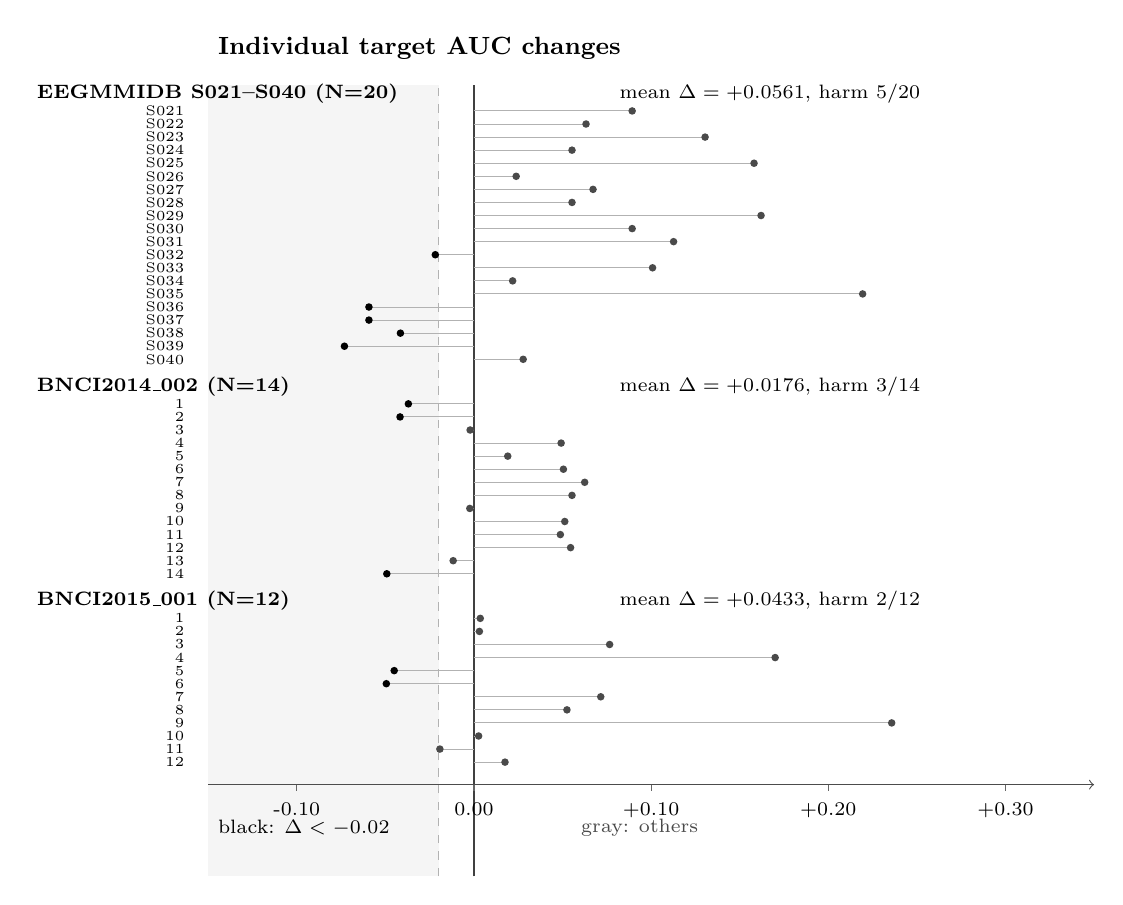
\begin{tikzpicture}[x=1cm,y=1cm]
\fill[gray!8] (2.300,1.68) rectangle (5.225,11.73);
\draw[dashed, gray!60] (5.225,1.68) -- (5.225,11.73);
\draw[black!75,line width=0.55pt] (5.675,1.68) -- (5.675,11.73);
\node[anchor=west,font=\small\bfseries] at (2.3,12.2) {Individual target AUC changes};
\node[anchor=west,font=\scriptsize\bfseries] at (0.0,11.620) {EEGMMIDB S021--S040 (N=20)};
\node[anchor=west,font=\scriptsize] at (7.4,11.620) {mean $\Delta=+0.0561$, harm 5/20};
\node[anchor=east,font=\tiny] at (2.12,11.400) {S021};
\draw[black!30,line width=0.35pt] (5.675,11.400) -- (7.684,11.400);
\fill[gray!58!black] (7.684,11.400) circle (0.048);
\node[anchor=east,font=\tiny] at (2.12,11.234) {S022};
\draw[black!30,line width=0.35pt] (5.675,11.234) -- (7.098,11.234);
\fill[gray!58!black] (7.098,11.234) circle (0.048);
\node[anchor=east,font=\tiny] at (2.12,11.068) {S023};
\draw[black!30,line width=0.35pt] (5.675,11.068) -- (8.610,11.068);
\fill[gray!58!black] (8.610,11.068) circle (0.048);
\node[anchor=east,font=\tiny] at (2.12,10.902) {S024};
\draw[black!30,line width=0.35pt] (5.675,10.902) -- (6.920,10.902);
\fill[gray!58!black] (6.920,10.902) circle (0.048);
\node[anchor=east,font=\tiny] at (2.12,10.736) {S025};
\draw[black!30,line width=0.35pt] (5.675,10.736) -- (9.232,10.736);
\fill[gray!58!black] (9.232,10.736) circle (0.048);
\node[anchor=east,font=\tiny] at (2.12,10.570) {S026};
\draw[black!30,line width=0.35pt] (5.675,10.570) -- (6.211,10.570);
\fill[gray!58!black] (6.211,10.570) circle (0.048);
\node[anchor=east,font=\tiny] at (2.12,10.404) {S027};
\draw[black!30,line width=0.35pt] (5.675,10.404) -- (7.187,10.404);
\fill[gray!58!black] (7.187,10.404) circle (0.048);
\node[anchor=east,font=\tiny] at (2.12,10.238) {S028};
\draw[black!30,line width=0.35pt] (5.675,10.238) -- (6.920,10.238);
\fill[gray!58!black] (6.920,10.238) circle (0.048);
\node[anchor=east,font=\tiny] at (2.12,10.072) {S029};
\draw[black!30,line width=0.35pt] (5.675,10.072) -- (9.321,10.072);
\fill[gray!58!black] (9.321,10.072) circle (0.048);
\node[anchor=east,font=\tiny] at (2.12,9.906) {S030};
\draw[black!30,line width=0.35pt] (5.675,9.906) -- (7.684,9.906);
\fill[gray!58!black] (7.684,9.906) circle (0.048);
\node[anchor=east,font=\tiny] at (2.12,9.740) {S031};
\draw[black!30,line width=0.35pt] (5.675,9.740) -- (8.210,9.740);
\fill[gray!58!black] (8.210,9.740) circle (0.048);
\node[anchor=east,font=\tiny] at (2.12,9.574) {S032};
\draw[black!30,line width=0.35pt] (5.675,9.574) -- (5.184,9.574);
\fill[black] (5.184,9.574) circle (0.048);
\node[anchor=east,font=\tiny] at (2.12,9.408) {S033};
\draw[black!30,line width=0.35pt] (5.675,9.408) -- (7.943,9.408);
\fill[gray!58!black] (7.943,9.408) circle (0.048);
\node[anchor=east,font=\tiny] at (2.12,9.242) {S034};
\draw[black!30,line width=0.35pt] (5.675,9.242) -- (6.166,9.242);
\fill[gray!58!black] (6.166,9.242) circle (0.048);
\node[anchor=east,font=\tiny] at (2.12,9.076) {S035};
\draw[black!30,line width=0.35pt] (5.675,9.076) -- (10.611,9.076);
\fill[gray!58!black] (10.611,9.076) circle (0.048);
\node[anchor=east,font=\tiny] at (2.12,8.910) {S036};
\draw[black!30,line width=0.35pt] (5.675,8.910) -- (4.341,8.910);
\fill[black] (4.341,8.910) circle (0.048);
\node[anchor=east,font=\tiny] at (2.12,8.744) {S037};
\draw[black!30,line width=0.35pt] (5.675,8.744) -- (4.341,8.744);
\fill[black] (4.341,8.744) circle (0.048);
\node[anchor=east,font=\tiny] at (2.12,8.578) {S038};
\draw[black!30,line width=0.35pt] (5.675,8.578) -- (4.741,8.578);
\fill[black] (4.741,8.578) circle (0.048);
\node[anchor=east,font=\tiny] at (2.12,8.412) {S039};
\draw[black!30,line width=0.35pt] (5.675,8.412) -- (4.030,8.412);
\fill[black] (4.030,8.412) circle (0.048);
\node[anchor=east,font=\tiny] at (2.12,8.246) {S040};
\draw[black!30,line width=0.35pt] (5.675,8.246) -- (6.300,8.246);
\fill[gray!58!black] (6.300,8.246) circle (0.048);
\node[anchor=west,font=\scriptsize\bfseries] at (0.0,7.900) {BNCI2014\_002 (N=14)};
\node[anchor=west,font=\scriptsize] at (7.4,7.900) {mean $\Delta=+0.0176$, harm 3/14};
\node[anchor=east,font=\tiny] at (2.12,7.680) {1};
\draw[black!30,line width=0.35pt] (5.675,7.680) -- (4.842,7.680);
\fill[black] (4.842,7.680) circle (0.048);
\node[anchor=east,font=\tiny] at (2.12,7.514) {2};
\draw[black!30,line width=0.35pt] (5.675,7.514) -- (4.736,7.514);
\fill[black] (4.736,7.514) circle (0.048);
\node[anchor=east,font=\tiny] at (2.12,7.348) {3};
\draw[black!30,line width=0.35pt] (5.675,7.348) -- (5.626,7.348);
\fill[gray!58!black] (5.626,7.348) circle (0.048);
\node[anchor=east,font=\tiny] at (2.12,7.182) {4};
\draw[black!30,line width=0.35pt] (5.675,7.182) -- (6.782,7.182);
\fill[gray!58!black] (6.782,7.182) circle (0.048);
\node[anchor=east,font=\tiny] at (2.12,7.016) {5};
\draw[black!30,line width=0.35pt] (5.675,7.016) -- (6.104,7.016);
\fill[gray!58!black] (6.104,7.016) circle (0.048);
\node[anchor=east,font=\tiny] at (2.12,6.850) {6};
\draw[black!30,line width=0.35pt] (5.675,6.850) -- (6.811,6.850);
\fill[gray!58!black] (6.811,6.850) circle (0.048);
\node[anchor=east,font=\tiny] at (2.12,6.684) {7};
\draw[black!30,line width=0.35pt] (5.675,6.684) -- (7.081,6.684);
\fill[gray!58!black] (7.081,6.684) circle (0.048);
\node[anchor=east,font=\tiny] at (2.12,6.518) {8};
\draw[black!30,line width=0.35pt] (5.675,6.518) -- (6.920,6.518);
\fill[gray!58!black] (6.920,6.518) circle (0.048);
\node[anchor=east,font=\tiny] at (2.12,6.352) {9};
\draw[black!30,line width=0.35pt] (5.675,6.352) -- (5.622,6.352);
\fill[gray!58!black] (5.622,6.352) circle (0.048);
\node[anchor=east,font=\tiny] at (2.12,6.186) {10};
\draw[black!30,line width=0.35pt] (5.675,6.186) -- (6.828,6.186);
\fill[gray!58!black] (6.828,6.186) circle (0.048);
\node[anchor=east,font=\tiny] at (2.12,6.020) {11};
\draw[black!30,line width=0.35pt] (5.675,6.020) -- (6.772,6.020);
\fill[gray!58!black] (6.772,6.020) circle (0.048);
\node[anchor=east,font=\tiny] at (2.12,5.854) {12};
\draw[black!30,line width=0.35pt] (5.675,5.854) -- (6.902,5.854);
\fill[gray!58!black] (6.902,5.854) circle (0.048);
\node[anchor=east,font=\tiny] at (2.12,5.688) {13};
\draw[black!30,line width=0.35pt] (5.675,5.688) -- (5.411,5.688);
\fill[gray!58!black] (5.411,5.688) circle (0.048);
\node[anchor=east,font=\tiny] at (2.12,5.522) {14};
\draw[black!30,line width=0.35pt] (5.675,5.522) -- (4.568,5.522);
\fill[black] (4.568,5.522) circle (0.048);
\node[anchor=west,font=\scriptsize\bfseries] at (0.0,5.176) {BNCI2015\_001 (N=12)};
\node[anchor=west,font=\scriptsize] at (7.4,5.176) {mean $\Delta=+0.0433$, harm 2/12};
\node[anchor=east,font=\tiny] at (2.12,4.956) {1};
\draw[black!30,line width=0.35pt] (5.675,4.956) -- (5.755,4.956);
\fill[gray!58!black] (5.755,4.956) circle (0.048);
\node[anchor=east,font=\tiny] at (2.12,4.790) {2};
\draw[black!30,line width=0.35pt] (5.675,4.790) -- (5.744,4.790);
\fill[gray!58!black] (5.744,4.790) circle (0.048);
\node[anchor=east,font=\tiny] at (2.12,4.624) {3};
\draw[black!30,line width=0.35pt] (5.675,4.624) -- (7.398,4.624);
\fill[gray!58!black] (7.398,4.624) circle (0.048);
\node[anchor=east,font=\tiny] at (2.12,4.458) {4};
\draw[black!30,line width=0.35pt] (5.675,4.458) -- (9.500,4.458);
\fill[gray!58!black] (9.500,4.458) circle (0.048);
\node[anchor=east,font=\tiny] at (2.12,4.292) {5};
\draw[black!30,line width=0.35pt] (5.675,4.292) -- (4.662,4.292);
\fill[black] (4.662,4.292) circle (0.048);
\node[anchor=east,font=\tiny] at (2.12,4.126) {6};
\draw[black!30,line width=0.35pt] (5.675,4.126) -- (4.562,4.126);
\fill[black] (4.562,4.126) circle (0.048);
\node[anchor=east,font=\tiny] at (2.12,3.960) {7};
\draw[black!30,line width=0.35pt] (5.675,3.960) -- (7.285,3.960);
\fill[gray!58!black] (7.285,3.960) circle (0.048);
\node[anchor=east,font=\tiny] at (2.12,3.794) {8};
\draw[black!30,line width=0.35pt] (5.675,3.794) -- (6.856,3.794);
\fill[gray!58!black] (6.856,3.794) circle (0.048);
\node[anchor=east,font=\tiny] at (2.12,3.628) {9};
\draw[black!30,line width=0.35pt] (5.675,3.628) -- (10.980,3.628);
\fill[gray!58!black] (10.980,3.628) circle (0.048);
\node[anchor=east,font=\tiny] at (2.12,3.462) {10};
\draw[black!30,line width=0.35pt] (5.675,3.462) -- (5.734,3.462);
\fill[gray!58!black] (5.734,3.462) circle (0.048);
\node[anchor=east,font=\tiny] at (2.12,3.296) {11};
\draw[black!30,line width=0.35pt] (5.675,3.296) -- (5.242,3.296);
\fill[gray!58!black] (5.242,3.296) circle (0.048);
\node[anchor=east,font=\tiny] at (2.12,3.130) {12};
\draw[black!30,line width=0.35pt] (5.675,3.130) -- (6.069,3.130);
\fill[gray!58!black] (6.069,3.130) circle (0.048);
\draw[->,black!70] (2.300,2.844) -- (13.550,2.844);
\draw[black!60] (3.425,2.844) -- (3.425,2.764);
\node[anchor=north,font=\scriptsize] at (3.425,2.734) {-0.10};
\draw[black!60] (5.675,2.844) -- (5.675,2.764);
\node[anchor=north,font=\scriptsize] at (5.675,2.734) {0.00};
\draw[black!60] (7.925,2.844) -- (7.925,2.764);
\node[anchor=north,font=\scriptsize] at (7.925,2.734) {+0.10};
\draw[black!60] (10.175,2.844) -- (10.175,2.764);
\node[anchor=north,font=\scriptsize] at (10.175,2.734) {+0.20};
\draw[black!60] (12.425,2.844) -- (12.425,2.764);
\node[anchor=north,font=\scriptsize] at (12.425,2.734) {+0.30};
\node[anchor=west,font=\scriptsize,black] at (2.300,2.294) {black: $\Delta<-0.02$};
\node[anchor=west,font=\scriptsize,gray!58!black] at (6.912,2.294) {gray: others};
\end{tikzpicture}
\caption{Paired participant-level target AUC differences between the frozen source participant-macro selector and the historical class-centred CovScore selector in three EEG cohorts. Five of 20, three of 14 and two of 12 participants, respectively, lost more than 0.02 AUC. The vertical reference line is zero, and the tinted region denotes the material-harm threshold. All three cohorts had been previously examined at project level; a within-run source lock does not turn the participant effects into externally preregistered confirmations. Historical Holm-adjusted results remain retrospective evidence. Points are descriptive and must not be treated as independent trials or a new confirmatory family.}
\label{fig:participant-harm-v10}
\end{figure*}


\subsection{The key prospective spectral-representation prediction fails}
On the separate untouched S041--S060 block, four prespecified
configurations compared WIDE231, FB8-1848, source-PCA-matched
FB8-231 and nuisance-augmented WIDE-1848. The primary
difference-in-differences for FB8-vs-WIDE under discrimination versus
Ledoit--Wolf regularisation was \(-0.07781\) AUC
(95\% [-0.12415,-0.03451], Holm \(p=0.01328\)).
The selection objective materially affected the representation
conclusion, but in the \emph{opposite} direction to the historical
claim that discrimination-oriented regularisation would reveal a
universal filter-bank advantage. Dimensionality-matched and nuisance
controls also contradicted a monotonic feature-dimension explanation.

\subsection{External path variation lacks a confirmed population lower bound}
Observed BNCI2014\_002 and BNCI2015\_001 AUC-path ranges were
0.03844 and 0.05011, with empirical \(\delta_{0.02}\) equal
to 0.91611 and 0.17519 per-dimension source NLL-regret units.
Post-outcome path-wide bootstrap oscillation radii were 0.04035
and 0.05923. In both cohorts, the resulting conservative
lower range bound is zero; a population-wide effect over 0.02
cannot be claimed from these data.

\begin{table*}[t]
\centering
\caption{Original v5 405-candidate target AUC path spreads and V11 translation-invariant simultaneous-path sensitivity. Observed ranges are exact reconstructions from the raw TRUE PRE-DATA external experiment outputs; ordinary 20,000-resample percentile intervals for an empirical max--min statistic are shown only for provenance, not as simultaneous population confidence intervals. \(q_{\mathrm{osc}}\) is the nominal 95th percentile of the paired-bootstrap error-path oscillation; \(L_{\mathrm{osc}}=\max(0,\text{observed span}-q_{\mathrm{osc}})\) conditions on the fixed studied cohorts and is post-outcome.}
\label{tab:validity-frontier}
\small
\begin{tabular}{lrrrrr}
\hline
Cohort & \(N\) & Observed span & Prior percentile interval & \(q_{\mathrm{osc}}\) & \(L_{\mathrm{osc}}\) \\
\hline
BNCI2014\_002 & 14 & 0.0384 & [0.0271, 0.0666] & 0.0403 & 0.0000 \\
BNCI2015\_001 & 12 & 0.0501 & [0.0224, 0.1034] & 0.0592 & 0.0000 \\
\hline
\end{tabular}

\vspace{1mm}
\footnotesize
Original observed \(\delta_{0.02}\) fidelity-regret budgets are 0.9161 and 0.1752 raw per-dimension source NLL units; neither path crosses the 0.02 AUC threshold after the V11 oscillation correction. A zero conservative lower bound is inconclusive, not proof of a flat population path. The bootstrap does not account for overlapping source-model refits or across-dataset sampling uncertainty. All quantities are descriptive and no new confirmatory hypothesis test is introduced.
\end{table*}



\subsection{Classical alternative and risk-boundary sensitivity}
A conventional six-component CSP plus logistic-regression
classifier supplies an additional reference in the two original
external BNCI cohorts. The source-macro tangent-LDA method
had descriptive mean AUC advantages of +0.04703 over CSP6 in
BNCI2014\_002 and +0.05360 in BNCI2015\_001. These
comparisons were conducted after the original primary frozen
test and are therefore labelled \emph{post-primary}; they do
not create two new confirmatory superiority tests. Their
participant-level bootstrap intervals were, respectively,
[-0.00291,0.09574] and [0.01220,0.10410], and both
included individuals for whom CSP was better. The latter
positive interval cannot repair the chronological limitation
of the post-primary comparison.

Absolute AUC improvements are not identical to a reliable
operating policy. For example, in the EEGMMIDB prospective
objective comparison five of 20 participants had a decrease
greater than 0.02 AUC relative to source covariance-NLL,
despite the mean positive effect. The other two primary
external BNCI cohorts had corresponding harmed-person counts
of three of 14 and two of 12. These are substantial rates
at the level of the observed participants. They do not
support a blanket recommendation that practitioners
should always replace covariance-oriented shrinkage with
source-macro selection.

A separate post-primary delete-one-source exercise fully
refitted the tangent reference and classifier, then reran
selection after omitting each development participant.
The mean contrast retained a positive direction in eight
of eight source omissions, but the selected discrimination
strength ranged between 0.4 and 0.95. This checks sensitivity
within the fixed, limited source pool. It is neither eight
new datasets nor evidence that the observed strength
generalises to a different acquisition site.

The two BNCI dataset-level positive means also should not be
misreported as replicated significant discoveries: the
Holm-corrected individual tests did not reject their null
hypotheses. Furthermore, participant-paired percentile
bootstraps over a selected 405-point regularisation path
can understate extrema-search uncertainty. Once a
post-outcome, translation-invariant whole-path error
oscillation is used as a sensitivity radius, the lower
span bound reaches zero in both external cohorts. The
data establish a reproducible \emph{observed} path spread,
not a positive, simultaneous population lower bound.
A more general fixed-threshold safety or calibration
claim would require new measurements and an evaluation
endpoint other than threshold-free AUC.


\subsection{Why source objective separation is not a validated switching rule}
\label{sec:source-target-not-predictor}
A limitation of objective-alignment scores is that they can appear
actionable without having been tested as prospective predictors of an
unseen person's gain. We therefore performed a clearly labelled
\emph{post-outcome descriptive} check using the \emph{original}
independently frozen Shin2017A score artifact. For each of the 29
outer participant folds, we read the original source-person AUC
path, its covariance-NLL path and the \emph{unchanged} held-person
model comparisons. Each source path was produced without the
held person's labels or feature statistics. The outer training pools
overlap heavily, so the 29 pairs do not constitute independent
source-to-deployment experiments.

The chosen discrimination criterion exceeded the AUC of the
source covariance-optimal candidate in all 29 folds, by
0.02605 source macro-AUC on average; it incurred a mean
source covariance-NLL cost of 0.72799 in the corresponding
per-dimension units. Both source-selected and
covariance-selected values came from the original same-grid
source validation. Yet that within-source separation was
\emph{not} proportional to the held-person benefit
(Fig.~\ref{fig:shin-posthoc-source-target}): the post-outcome
rank association of source AUC advantage with the target
AUC contrast was descriptively negative (Spearman
$\rho=-0.543$). A conventional independent-pairs
$p$-value is invalid here because most folds reuse the same
source participants. We make no general predictive or causal
claim from this exploratory association, and specify no
decision threshold using target outcomes.

\begin{table}[tb]
\centering
\small
\caption{Post-outcome robustness of the \emph{separately frozen}
Shin2017A (29 people). All contrasts refer to the same
original participant score family. Monte Carlo checks were
repeated for integrity only; the original family-adjusted
$p$-values remain the primary inference.}
\label{tab:shin-posthoc-robust}
\begin{tabular}{lcc}
\toprule
Post-outcome summary & vs Cov-NLL & vs Ledoit--Wolf\\
\midrule
Mean $\Delta$AUC (original) & +0.02222 & +0.04866\\
Median $\Delta$AUC & +0.01778 & +0.04667\\
10\% trimmed mean & +0.02062 & +0.04507\\
Minimum 1-person-deletion mean & +0.01750 & +0.04254\\
Maximum 1-person-deletion mean & +0.02623 & +0.05278\\
People harmed by $>0.02$ AUC & 5/29 & 3/29\\
\bottomrule
\end{tabular}
\end{table}

Every one-person omission retained a positive cohort mean,
but even a bootstrap or deletion check conditional on these
overlapping source fits does not establish a participant-safe
adaptive policy. In particular, the harmed fraction against
covariance-NLL was 17.2\% (5/29), with an exploratory Wilson
95\% interval of approximately 7.6--34.5\%;
the comparable Ledoit--Wolf fraction was 10.3\% (3/29).
Those intervals do not account for variation across new
EEG acquisition sites or independently retrained source pools.
They express uncertainty under a much narrower sampling
model, and are not medical safety intervals.

\begin{figure}[tb]
\centering
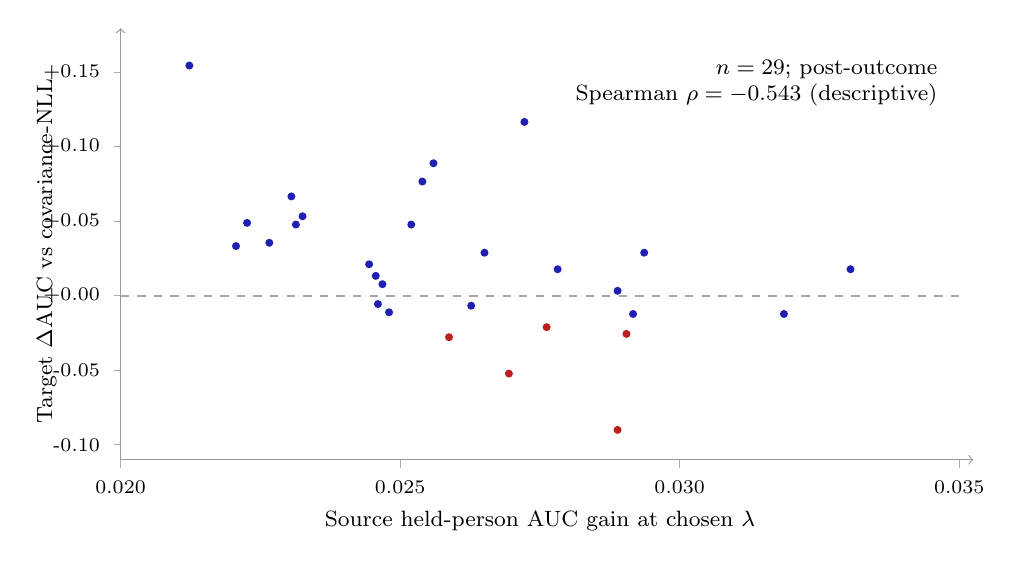
\begin{tikzpicture}[x=1cm,y=1cm]
\draw[->,gray!80] (1.450,1.000) -- (12.280,1.000);
\draw[->,gray!80] (1.450,1.000) -- (1.450,6.480);
\draw[dashed,gray!70,line width=.55pt] (1.450,3.082) -- (12.100,3.082);
\draw[gray!65] (1.360,1.189) -- (1.450,1.189);
\node[anchor=east,font=\scriptsize] at (1.310,1.189) {-0.10};
\draw[gray!65] (1.360,2.136) -- (1.450,2.136);
\node[anchor=east,font=\scriptsize] at (1.310,2.136) {-0.05};
\draw[gray!65] (1.360,3.082) -- (1.450,3.082);
\node[anchor=east,font=\scriptsize] at (1.310,3.082) {+0.00};
\draw[gray!65] (1.360,4.029) -- (1.450,4.029);
\node[anchor=east,font=\scriptsize] at (1.310,4.029) {+0.05};
\draw[gray!65] (1.360,4.975) -- (1.450,4.975);
\node[anchor=east,font=\scriptsize] at (1.310,4.975) {+0.10};
\draw[gray!65] (1.360,5.921) -- (1.450,5.921);
\node[anchor=east,font=\scriptsize] at (1.310,5.921) {+0.15};
\draw[gray!65] (1.450,1.000) -- (1.450,0.900);
\node[anchor=north,font=\scriptsize] at (1.450,0.850) {0.020};
\draw[gray!65] (5.000,1.000) -- (5.000,0.900);
\node[anchor=north,font=\scriptsize] at (5.000,0.850) {0.025};
\draw[gray!65] (8.550,1.000) -- (8.550,0.900);
\node[anchor=north,font=\scriptsize] at (8.550,0.850) {0.030};
\draw[gray!65] (12.100,1.000) -- (12.100,0.900);
\node[anchor=north,font=\scriptsize] at (12.100,0.850) {0.035};
\node[font=\footnotesize,align=center] at (6.775,0.220) {Source held-person AUC gain at chosen $\lambda$};
\node[rotate=90,font=\footnotesize] at (0.510,3.650) {Target $\Delta$AUC vs covariance-NLL};
\fill[blue!65!black,opacity=.88] (10.719,3.419) circle (1.45pt);
\fill[blue!65!black,opacity=.88] (5.423,4.765) circle (1.45pt);
\fill[blue!65!black,opacity=.88] (3.056,4.008) circle (1.45pt);
\fill[blue!65!black,opacity=.88] (3.619,4.344) circle (1.45pt);
\fill[blue!65!black,opacity=.88] (3.676,3.987) circle (1.45pt);
\fill[blue!65!black,opacity=.88] (3.338,3.755) circle (1.45pt);
\fill[red!70!black,opacity=.88] (6.381,2.094) circle (1.45pt);
\fill[blue!65!black,opacity=.88] (2.323,6.006) circle (1.45pt);
\fill[blue!65!black,opacity=.88] (7.761,3.145) circle (1.45pt);
\fill[blue!65!black,opacity=.88] (4.859,2.872) circle (1.45pt);
\fill[blue!65!black,opacity=.88] (8.099,3.629) circle (1.45pt);
\fill[red!70!black,opacity=.88] (7.874,2.598) circle (1.45pt);
\fill[red!70!black,opacity=.88] (7.761,1.379) circle (1.45pt);
\fill[blue!65!black,opacity=.88] (9.874,2.851) circle (1.45pt);
\fill[blue!65!black,opacity=.88] (5.141,3.987) circle (1.45pt);
\fill[blue!65!black,opacity=.88] (6.071,3.629) circle (1.45pt);
\fill[blue!65!black,opacity=.88] (4.718,2.977) circle (1.45pt);
\fill[blue!65!black,opacity=.88] (5.902,2.956) circle (1.45pt);
\fill[blue!65!black,opacity=.88] (4.690,3.335) circle (1.45pt);
\fill[blue!65!black,opacity=.88] (2.915,3.713) circle (1.45pt);
\fill[red!70!black,opacity=.88] (5.620,2.556) circle (1.45pt);
\fill[blue!65!black,opacity=.88] (4.606,3.482) circle (1.45pt);
\fill[blue!65!black,opacity=.88] (4.775,3.229) circle (1.45pt);
\fill[blue!65!black,opacity=.88] (7.958,2.851) circle (1.45pt);
\fill[blue!65!black,opacity=.88] (7.000,3.419) circle (1.45pt);
\fill[blue!65!black,opacity=.88] (3.760,4.092) circle (1.45pt);
\fill[blue!65!black,opacity=.88] (6.578,5.290) circle (1.45pt);
\fill[blue!65!black,opacity=.88] (5.282,4.533) circle (1.45pt);
\fill[red!70!black,opacity=.88] (6.860,2.683) circle (1.45pt);
\node[anchor=north east,font=\footnotesize,fill=white,inner sep=2pt,align=right] at (11.900,6.150) {$n=29$; post-outcome\\Spearman $\rho=-0.543$ (descriptive)};
\end{tikzpicture}
\caption{Exploratory, non-predictive sensitivity analysis on the 29 original Shin2017A frozen folds. Source-only held-source AUC advantage is compared against realised held-person AUC benefit. Red points denote participants harmed by more than 0.02 AUC. Training-source pools strongly overlap across outer folds, so these points cannot support an independent-samples correlation test or a prospective switching threshold. These observations were analysed after the original outcome release.}
\label{fig:shin-posthoc-source-target}
\end{figure}



\section{Discussion}
The study establishes a practical inference hazard inside the tested
covariance/tangent-space LDA family: an estimation-targeted regulariser
can select a different region from a discrimination-targeted rule, with
meaningful changes to held-person performance and to which
representation appears favourable. The problem is not a previously
unknown mathematical property of RDA \cite{friedman1989}.
It is the documented, prospectively tested consequence under a strictly
source-only EEG evaluation contract. Reporting the source criterion and
its selected strength should accompany conclusions drawn from the
accuracy of spectral representations.

The evidence is heterogeneous rather than universal. Two independently
pre-data-frozen BNCI cohorts have positive mean directions but individually
non-significant adjusted tests. Shin2017A has its own pre-outcome family.
The cross-representation intervention directly falsifies the originally
expected filter-bank improvement, and none of the proposed follow-up
source-only tail/fidelity heuristics has passed a promotion rule.
The post-outcome frontier correction removes the earlier population
span interpretation. These adverse findings constrain the contribution
and should remain visible rather than be suppressed.

The new source-only regret/rotation diagnostic is a measurement instrument,
not a validated alarm threshold or a new covariance estimator. Its
prospective predictive value and decision safety remain untested. Nor do
these offline AUC results establish clinically relevant operating thresholds,
reduced labelled calibration burden or superior modern deep EEG decoding.
The data contain few independent acquisition laboratories, while
test-participant bootstrap inference does not capture overlapping
source-fit variation or future domain shifts. Broad clinical claims
would require a separate pre-registered device/session/threshold utility study.

\section{Conclusion}
Covariance-fidelity and held-participant discrimination objectives selected
distinct regularisation regions, with a prospectively verified mean target
effect in a zero-target EEG pipeline. External replication qualifies the
strength of inference, and a separate prospective falsification shows that
the regularisation objective can alter the scientific interpretation
of a spectral-representation comparison. The result motivates explicit
reporting and sensitivity analysis, not a universal multiplier or
participant-safe deployment policy.

\section*{Statements and Declarations}
\textbf{Data availability:} The EEG cohorts are publicly distributed.
Original participant score receipts, repository commit hashes and code
availability must be confirmed in the final submission package.

\textbf{Author contribution, funding, competing interests, ethics and
AI-assisted writing:} To be completed and confirmed by all authors before
publisher upload. No declaration is made on an author's behalf.

\bibliographystyle{unsrt}
\bibliography{references_v10}
\end{document}
